\documentclass[aspectratio=169, 11pt]{beamer}

% ── Theme ──────────────────────────────────────────────────
\usetheme{metropolis}
\usecolortheme{default}

\definecolor{tumblue}{RGB}{0, 101, 189}
\definecolor{tumgray}{RGB}{88, 88, 90}
\definecolor{tumlightblue}{RGB}{100, 160, 220}
\definecolor{tumred}{RGB}{196, 7, 27}
\definecolor{casea}{RGB}{39, 174, 96}
\definecolor{caseb}{RGB}{241, 196, 15}
\definecolor{casec}{RGB}{231, 76, 60}

\setbeamercolor{frametitle}{bg=tumblue, fg=white}
\setbeamercolor{title}{fg=tumblue}
\setbeamercolor{alerted text}{fg=tumred}
\setbeamercolor{block title}{bg=tumblue, fg=white}
\setbeamercolor{progress bar}{fg=tumblue}

\usepackage[T1]{fontenc}
\usepackage[utf8]{inputenc}
\usepackage{graphicx}
\usepackage{booktabs}
\usepackage{tikz}
\usetikzlibrary{arrows.meta, positioning, shapes.geometric, calc}
\usepackage{amsmath, amssymb}
\usepackage{xcolor}

\setbeamertemplate{navigation symbols}{}
\setbeamertemplate{footline}[frame number]

% ── Title ──────────────────────────────────────────────────
\title{RAG-Based AI Tutor for the\\Tunisian Baccalaureate in Mathematics}
\subtitle{Bachelor's Thesis}
\author{Rayen Fdhili}
\institute{Technical University of Munich\\
Supervisor: Frederic Mrozinski \quad Professor: Apl.\ Prof.\ Dr.\ Georg Groh}
\date{April 2, 2026}

\begin{document}

% ══════════════════════════════════════════════════════════════
% SLIDE 1: TITLE
% ══════════════════════════════════════════════════════════════
\begin{frame}[plain]
\maketitle
\end{frame}


% ══════════════════════════════════════════════════════════════
% SLIDE 2: OUTLINE
% ══════════════════════════════════════════════════════════════
\begin{frame}{Outline}
\begin{enumerate}
    \item Motivation \& Problem
    \item Data Collection
    \item Building the System
    \item The Three Approaches
    \item Evaluation
    \item Results \& Discussion
    \item Conclusion
\end{enumerate}
\end{frame}


% ══════════════════════════════════════════════════════════════
% SLIDE 3: MOTIVATION
% ══════════════════════════════════════════════════════════════
\begin{frame}{Why This Project?}

The Tunisian Baccalaureate (Section Maths) is \textbf{high-stakes}: it determines
university access for 40{,}000+ students every year.

\bigskip

\textbf{The problem:}
\begin{itemize}
    \item Private tutoring is expensive and not available everywhere
    \item Generic AI tools (ChatGPT, etc.) don't know the Tunisian curriculum
    \item They use methods that are \alert{forbidden} in the Tunisian program \\
          (e.g.\ L'H\^opital's rule, Taylor series, matrix diagonalization)
    \item They don't write answers in the official Bac correction style
\end{itemize}

\bigskip

\textbf{Goal:} Build an AI tutor that answers \textit{strictly} within the
Tunisian Bac curriculum and mimics the official correction style.

\end{frame}


% ══════════════════════════════════════════════════════════════
% SLIDE 4: CONSTRAINTS
% ══════════════════════════════════════════════════════════════
\begin{frame}{Constraints I Had to Work With}

\begin{columns}[T]
\begin{column}{0.48\textwidth}
\textbf{Curriculum constraints}
\begin{itemize}
    \item 10 specific chapters
    \item Strict list of allowed methods
    \item Official redaction style:\\
          ``On a\ldots'', ``Or\ldots'', ``Donc\ldots''
    \item French academic language
\end{itemize}
\end{column}
\begin{column}{0.48\textwidth}
\textbf{Technical constraints}
\begin{itemize}
    \item Math content (LaTeX notation)
    \item Mixed languages (French + Derja)
    \item No existing digitized corpus
    \item Limited corpus size
\end{itemize}
\end{column}
\end{columns}

\end{frame}


% ══════════════════════════════════════════════════════════════
% SLIDE 5: DATA COLLECTION
% ══════════════════════════════════════════════════════════════
\begin{frame}{Step 1: Getting the Data}

\begin{columns}[T]
\begin{column}{0.55\textwidth}

I traveled to Tunisia and collected raw materials:
\begin{itemize}
    \item Official Bac exams with corrections (2010--2024)
    \item Series exercises from high school teachers
    \item Course material (textbook chapters)
\end{itemize}

\bigskip

Scanned everything with my phone camera.

\bigskip

\textbf{Result:} 624 raw files (PDFs and images) organized by chapter, uploaded to Google Cloud Storage.

\end{column}
\begin{column}{0.40\textwidth}
% placeholder for a photo of scanned exams
\begin{center}
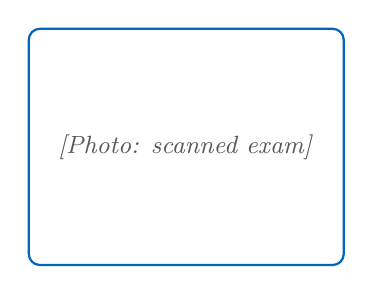
\begin{tikzpicture}
  \draw[tumblue, thick, rounded corners] (0,0) rectangle (4,3);
  \node[tumgray] at (2,1.5) {\small \textit{[Photo: scanned exam]}};
\end{tikzpicture}

\vspace{0.3cm}
\small 10 chapters $\times$ 3 types\\
(exams, series, cours)
\end{center}
\end{column}
\end{columns}

\end{frame}


% ══════════════════════════════════════════════════════════════
% SLIDE 6: DIGITIZATION
% ══════════════════════════════════════════════════════════════
\begin{frame}{Step 2: Digitization (Images $\to$ LaTeX)}

\begin{center}
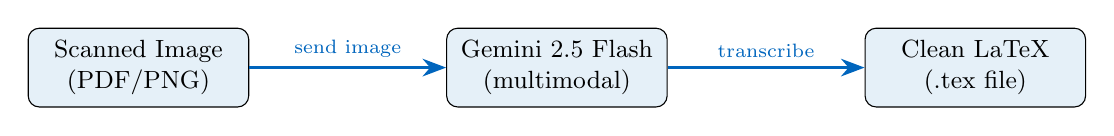
\begin{tikzpicture}[
    node distance=1.2cm,
    box/.style={draw, rounded corners, minimum width=2.8cm, minimum height=1cm,
                align=center, font=\small},
    arr/.style={-{Stealth[length=3mm]}, thick, tumblue}
]
    \node[box, fill=tumblue!10] (img) {Scanned Image\\(PDF/PNG)};
    \node[box, fill=tumblue!10, right=2.5cm of img] (gemini) {Gemini 2.5 Flash\\(multimodal)};
    \node[box, fill=tumblue!10, right=2.5cm of gemini] (tex) {Clean LaTeX\\(.tex file)};

    \draw[arr] (img) -- (gemini) node[midway, above, font=\scriptsize] {send image};
    \draw[arr] (gemini) -- (tex) node[midway, above, font=\scriptsize] {transcribe};
\end{tikzpicture}
\end{center}

\bigskip

\begin{itemize}
    \item Used Gemini's multimodal capability to ``read'' handwritten/printed math
    \item French prompt telling it to preserve the exact Tunisian notation
    \item Automatic retry with exponential backoff on API failures
    \item Skips already-digitized files (cost-safe)
\end{itemize}

\bigskip
\textbf{Quality:} 5.4\% Character Error Rate, 97.1\% LaTeX math accuracy
(measured against manually corrected references).

\end{frame}


% ══════════════════════════════════════════════════════════════
% SLIDE 7: DATABASE CONSTRUCTION
% ══════════════════════════════════════════════════════════════
\begin{frame}{Step 3: Building the Vector Database}

\begin{center}
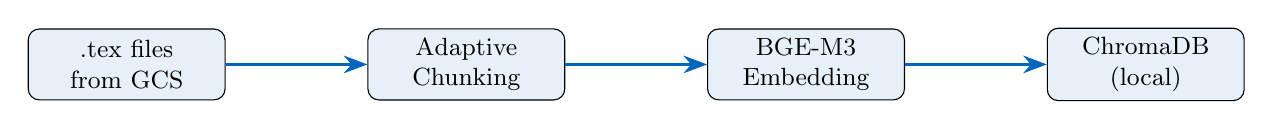
\begin{tikzpicture}[
    node distance=0.8cm,
    box/.style={draw, rounded corners, minimum width=2.5cm, minimum height=0.9cm,
                align=center, font=\small},
    arr/.style={-{Stealth[length=3mm]}, thick, tumblue}
]
    \node[box, fill=tumblue!10] (tex) {.tex files\\from GCS};
    \node[box, fill=tumblue!10, right=1.8cm of tex] (chunk) {Adaptive\\Chunking};
    \node[box, fill=tumblue!10, right=1.8cm of chunk] (embed) {BGE-M3\\Embedding};
    \node[box, fill=tumblue!10, right=1.8cm of embed] (db) {ChromaDB\\(local)};

    \draw[arr] (tex) -- (chunk);
    \draw[arr] (chunk) -- (embed);
    \draw[arr] (embed) -- (db);
\end{tikzpicture}
\end{center}

\bigskip

\textbf{Adaptive chunking:}
\begin{itemize}
    \item Corrections $\to$ 1500 chars (preserve exercise boundaries)
    \item Course material $\to$ 3000 chars (keep theorem context)
\end{itemize}

\textbf{Rich metadata} per chunk: chapter, year, doc type, is\_solution, exercise key

\textbf{BGE-M3 embeddings:} multilingual (French + Derja + LaTeX), 1024 dimensions

\bigskip
\textbf{Result:} 903 chunks from 624 files, fully searchable.

\end{frame}


% ══════════════════════════════════════════════════════════════
% SLIDE 8: THREE APPROACHES OVERVIEW
% ══════════════════════════════════════════════════════════════
\begin{frame}{The Three Approaches}

\begin{center}
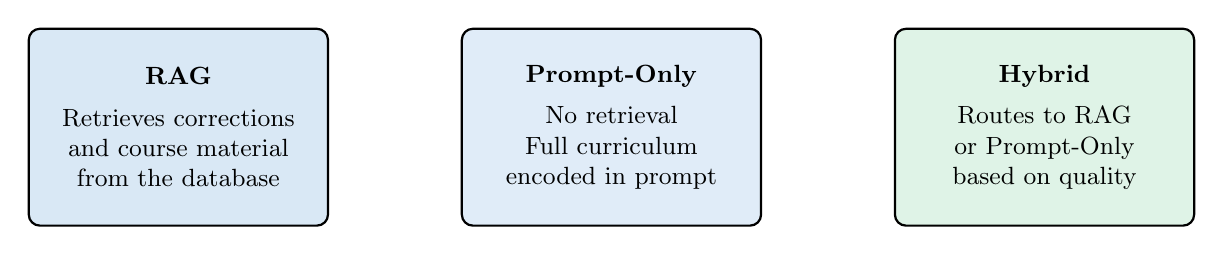
\begin{tikzpicture}[
    sysbox/.style={draw, rounded corners, minimum width=3.8cm, minimum height=2.5cm,
                   align=center, font=\small, thick},
]
    \node[sysbox, fill=tumblue!15] (rag) at (0,0) {
        \textbf{RAG}\\[4pt]
        Retrieves corrections\\
        and course material\\
        from the database
    };
    \node[sysbox, fill=tumlightblue!20] (po) at (5.5,0) {
        \textbf{Prompt-Only}\\[4pt]
        No retrieval\\
        Full curriculum\\
        encoded in prompt
    };
    \node[sysbox, fill=casea!15] (hyb) at (11,0) {
        \textbf{Hybrid}\\[4pt]
        Routes to RAG\\
        or Prompt-Only\\
        based on quality
    };
\end{tikzpicture}
\end{center}

\bigskip

All three use the \textbf{same Gemini model} with the \textbf{same temperature} (0.15).

The \textit{only variable} is where the knowledge comes from.

\end{frame}


% ══════════════════════════════════════════════════════════════
% SLIDE 9: RAG ENGINE
% ══════════════════════════════════════════════════════════════
\begin{frame}{RAG Engine: Two-Stage Retrieval}

\begin{center}
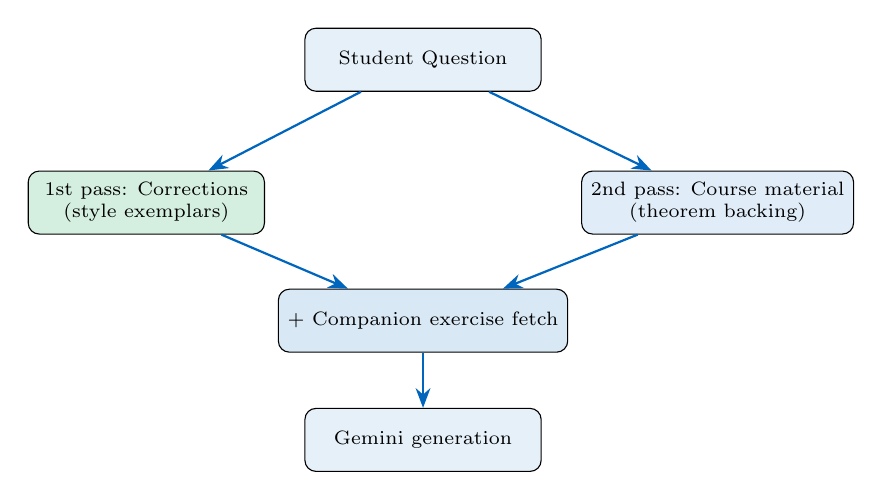
\begin{tikzpicture}[
    node distance=0.6cm,
    box/.style={draw, rounded corners, minimum width=3cm, minimum height=0.8cm,
                align=center, font=\scriptsize},
    arr/.style={-{Stealth[length=2.5mm]}, thick, tumblue}
]
    \node[box, fill=tumblue!10] (q) {Student Question};

    \node[box, fill=casea!20, below left=1cm and 0.5cm of q] (p1) {1st pass: Corrections\\(style exemplars)};
    \node[box, fill=tumlightblue!20, below right=1cm and 0.5cm of q] (p2) {2nd pass: Course material\\(theorem backing)};

    \node[box, fill=tumblue!15, below=2.5cm of q] (comp) {+ Companion exercise fetch};
    \node[box, fill=tumblue!10, below=0.7cm of comp] (gen) {Gemini generation};

    \draw[arr] (q) -- (p1);
    \draw[arr] (q) -- (p2);
    \draw[arr] (p1) -- (comp);
    \draw[arr] (p2) -- (comp);
    \draw[arr] (comp) -- (gen);
\end{tikzpicture}
\end{center}

\begin{itemize}
    \item \textbf{1st pass:} searches corrections (is\_solution=true) for \textit{redaction style}
    \item \textbf{2nd pass:} searches course material, scoped to the relevant chapter(s)
    \item \textbf{Companion fetch:} pairs each correction with its exercise statement
    \item ``Monsieur Tounsi'' persona with Derja sandwich and anti-hallucination rules
\end{itemize}

\end{frame}


% ══════════════════════════════════════════════════════════════
% SLIDE 10: PROMPT-ONLY ENGINE
% ══════════════════════════════════════════════════════════════
\begin{frame}{Prompt-Only: The Baseline}

No database. No embeddings. Just a very carefully written prompt.

\bigskip

The system prompt encodes:
\begin{enumerate}
    \item The full curriculum (10 chapters with key theorems)
    \item A list of \alert{forbidden methods} (L'H\^opital, Taylor, etc.)
    \item The official Bac redaction style
    \item Self-verification rules
    \item Hallucination control (``don't cite specific exam numbers unless certain'')
    \item Confidence calibration
\end{enumerate}

\bigskip

\textbf{Why build this?}

To answer the question: \textit{does retrieval actually help, or is a good prompt enough?}

\end{frame}


% ══════════════════════════════════════════════════════════════
% SLIDE 11: HYBRID ENGINE
% ══════════════════════════════════════════════════════════════
\begin{frame}{Hybrid Engine: Adaptive Routing}

\begin{center}
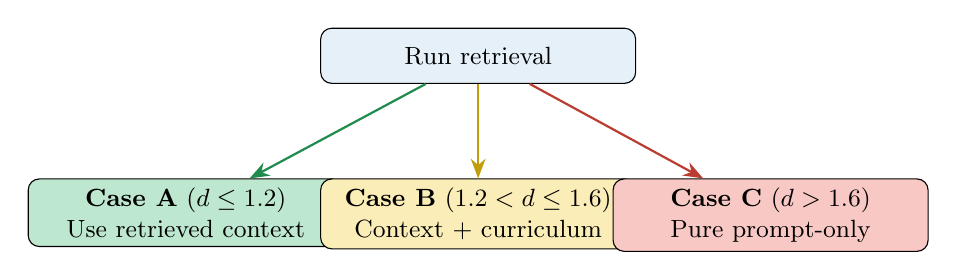
\begin{tikzpicture}[
    node distance=0.5cm,
    box/.style={draw, rounded corners, minimum width=4cm, minimum height=0.7cm,
                align=center, font=\small},
    arr/.style={-{Stealth[length=2.5mm]}, thick}
]
    \node[box, fill=tumblue!10] (q) {Run retrieval};
    \node[box, fill=casea!30, below left=1.2cm and -0.3cm of q] (a)
        {\textbf{Case A} ($d \leq 1.2$)\\Use retrieved context};
    \node[box, fill=caseb!30, below=1.2cm of q] (b)
        {\textbf{Case B} ($1.2 < d \leq 1.6$)\\Context + curriculum};
    \node[box, fill=casec!30, below right=1.2cm and -0.3cm of q] (c)
        {\textbf{Case C} ($d > 1.6$)\\Pure prompt-only};

    \draw[arr, casea!80!black] (q) -- (a);
    \draw[arr, caseb!80!black] (q) -- (b);
    \draw[arr, casec!80!black] (q) -- (c);
\end{tikzpicture}
\end{center}

\bigskip

\begin{itemize}
    \item Always attempts retrieval first
    \item Uses the best L2 distance to decide which case
    \item \textbf{Case B} is the novel contribution: merges both knowledge sources,
          tells the model to signal which source it's using
    \item Graceful degradation: never fails, just adapts
\end{itemize}

\end{frame}


% ══════════════════════════════════════════════════════════════
% SLIDE 12: EVALUATION METHODOLOGY
% ══════════════════════════════════════════════════════════════
\begin{frame}{How I Evaluated: Blind Human Grading}

\textbf{20 questions} across 5 categories:

\begin{center}
\small
\begin{tabular}{cl}
\toprule
\textbf{Cat.} & \textbf{Description} \\
\midrule
A (5) & Direct Bac-style (should be in the corpus) \\
B (5) & Novel problems (same topics, new exercises) \\
C (3) & Informal student questions (coaching mode) \\
D (2) & Tunisian Derja (mixed language) \\
E (4) & Out-of-scope (should be refused) \\
\bottomrule
\end{tabular}
\end{center}

\bigskip

\textbf{Blind grading} by a Tunisian Bac math teacher:
\begin{itemize}
    \item Sees ``Syst\`eme X / Y / Z'' --- doesn't know which system is which
    \item 4 criteria (0--5 each): correctness, clarity, pedagogy, Bac style
    \item Guardrail questions graded separately (PASS/FAIL)
\end{itemize}

\end{frame}


% ══════════════════════════════════════════════════════════════
% SLIDE 13: MAIN RESULTS
% ══════════════════════════════════════════════════════════════
\begin{frame}{Results: Overall Scores}

\begin{center}
\begin{tabular}{lrrr}
\toprule
\textbf{Criterion} & \textbf{RAG} & \textbf{Prompt-Only} & \textbf{Hybrid} \\
\midrule
Mathematical Correctness & 3.27 & \textbf{4.47} & 3.33 \\
Reasoning Clarity        & 3.40 & \textbf{4.47} & 3.27 \\
Pedagogical Quality      & 3.07 & \textbf{4.27} & 3.07 \\
Bac Style Adherence      & 3.13 & \textbf{4.07} & 3.33 \\
\midrule
\textbf{Mean}            & 3.22 & \textbf{4.32} & 3.25 \\
\bottomrule
\end{tabular}
\end{center}

\bigskip

\begin{center}
\large
Prompt-Only wins: \textbf{4.32/5} \quad vs.\quad RAG: 3.22 \quad Hybrid: 3.25
\end{center}

\bigskip

All three systems passed all 4 guardrail tests (out-of-scope refusal).

\end{frame}


% ══════════════════════════════════════════════════════════════
% SLIDE 14: WHY PROMPT-ONLY WON
% ══════════════════════════════════════════════════════════════
\begin{frame}{Why Did Prompt-Only Win?}

\textbf{The retrieval was the bottleneck, not the generation.}

\bigskip

\begin{columns}[T]
\begin{column}{0.48\textwidth}
\textbf{What went wrong with retrieval:}
\begin{itemize}
    \item 60\% chapter match --- retrieved docs were often from the wrong chapter
    \item Multi-topic Bac compilations dominated the results
    \item Low distance $\neq$ correct topic
\end{itemize}
\end{column}
\begin{column}{0.48\textwidth}
\textbf{Why Prompt-Only worked:}
\begin{itemize}
    \item Gemini already knows the math
    \item The prompt gave it the exact structure and style
    \item No risk of irrelevant context confusing the model
\end{itemize}
\end{column}
\end{columns}

\bigskip

\textbf{Key insight:} With a small corpus (624 files), retrieval introduces more noise
than signal. RAG becomes valuable when the corpus is large enough to reliably
find the right content.

\end{frame}


% ══════════════════════════════════════════════════════════════
% SLIDE 15: EMBEDDING ANALYSIS
% ══════════════════════════════════════════════════════════════
\begin{frame}{Embedding Model Choice: BGE-M3 vs Google}

\begin{center}
\small
\begin{tabular}{lrr}
\toprule
\textbf{Metric} & \textbf{BGE-M3} & \textbf{Google} \\
\midrule
Dimension & 1024 & 768 \\
Mean best L2 distance & 0.69 & 0.51 \\
All queries in Case A & 15/15 & 15/15 \\
\midrule
\multicolumn{3}{c}{\textit{Variable sensitivity ($u_n \to v_n$)}} \\
\midrule
Mean top-3 overlap & \textbf{44\%} & 11\% \\
Same top-1 document & \textbf{5/6} & 3/6 \\
\bottomrule
\end{tabular}
\end{center}

\bigskip

Google has lower distances (looks better on paper), but BGE-M3 is
\textbf{4$\times$ more consistent} when you just change a variable name.

\bigskip

For a math tutor, \textit{consistency matters more than raw distance}.

\end{frame}


% ══════════════════════════════════════════════════════════════
% SLIDE 16: PER-CATEGORY
% ══════════════════════════════════════════════════════════════
\begin{frame}{Results by Category}

\begin{center}
\begin{tabular}{llrrr}
\toprule
& \textbf{Category} & \textbf{RAG} & \textbf{Prompt-Only} & \textbf{Hybrid} \\
\midrule
A & Direct Bac-style    & 2.70 & \textbf{4.25} & 3.00 \\
B & Novel problems      & 3.30 & \textbf{4.50} & 3.25 \\
C & Informal (coaching) & 3.58 & \textbf{4.17} & 3.42 \\
D & Derja (mixed lang.) & 3.88 & \textbf{4.38} & 3.63 \\
\bottomrule
\end{tabular}
\end{center}

\bigskip

\begin{itemize}
    \item \textbf{Category D} (Derja): smallest gap --- BGE-M3 handles multilingual well
    \item \textbf{Category A} (direct Bac): largest gap --- retrieval found wrong chapters
    \item \textbf{Category C} (coaching): all systems do reasonably well in pedagogical mode
\end{itemize}

\end{frame}


% ══════════════════════════════════════════════════════════════
% SLIDE 17: QUALITATIVE EXAMPLE
% ══════════════════════════════════════════════════════════════
\begin{frame}{A Concrete Example}

\textbf{Question (B02):} ``Urne: 5 blanches, 3 noires. Tirage successif
sans remise de 3 boules. Calculer $P$(exactement 2 blanches).''

\bigskip

\begin{description}
    \item[\textcolor{tumblue}{RAG}] Best distance = 0.40 (looks great!).
        But the retrieved correction was about \textit{simultaneous} draws,
        not \textit{sequential} draws. Gave a brief, partially wrong answer.

    \item[\textcolor{casea}{Prompt-Only}] Correctly identified sequential draws,
        worked through both sub-questions with explicit combinatorial reasoning.

    \item[\textcolor{caseb}{Hybrid}] Referenced the wrong context (simultaneous draws),
        couldn't override its Case A instructions.
\end{description}

\bigskip

\textbf{Lesson:} Low retrieval distance $\neq$ correct content.

\end{frame}


% ══════════════════════════════════════════════════════════════
% SLIDE 18: LIMITATIONS & FUTURE WORK
% ══════════════════════════════════════════════════════════════
\begin{frame}{Limitations \& Future Work}

\textbf{Limitations:}
\begin{itemize}
    \item Small corpus (624 files) --- RAG needs more data to shine
    \item 1 evaluator (1 teacher, 15 graded questions)
    \item Thresholds (1.2, 1.6) are heuristic, not optimized
    \item No student user study yet
\end{itemize}

\bigskip

\textbf{Future work:}
\begin{itemize}
    \item Scale the corpus: more years, more chapters, more teachers' series
    \item Experiment with threshold tuning
    \item Add chapter-level re-ranking (not just distance)
    \item Fine-tune embeddings on Tunisian math data
    \item Deploy and test with real students
\end{itemize}

\end{frame}


% ══════════════════════════════════════════════════════════════
% SLIDE 19: CONCLUSION
% ══════════════════════════════════════════════════════════════
\begin{frame}{Conclusion}

\begin{enumerate}
    \item Built a \textbf{complete RAG pipeline} from raw scanned exams to
          a working AI tutor for the Tunisian Bac

    \item Compared \textbf{three approaches} (RAG, Prompt-Only, Hybrid)
          under controlled conditions

    \item \textbf{Prompt-Only outperformed RAG} (4.32 vs.\ 3.22/5) at this
          corpus scale --- retrieval introduced noise

    \item The \textbf{Hybrid approach} provides graceful degradation but
          couldn't overcome retrieval quality issues

    \item \textbf{Corpus size is the bottleneck}: with more data,
          RAG's advantage should emerge
\end{enumerate}

\bigskip

\begin{center}
\textit{The system is ready --- it just needs more data.}
\end{center}

\end{frame}


% ══════════════════════════════════════════════════════════════
% SLIDE 20: THANK YOU
% ══════════════════════════════════════════════════════════════
\begin{frame}[plain]
\begin{center}
\vspace{2cm}
{\Large \textbf{Thank you!}}

\bigskip

{\large Questions?}

\vspace{1.5cm}

{\small Rayen Fdhili \quad $\cdot$ \quad TUM \quad $\cdot$ \quad April 2026}
\end{center}
\end{frame}

\end{document}
